\documentclass[10pt,a4paper]{article}
\usepackage[utf8]{inputenc}
%\usepackage[spanish]{babel}
\usepackage{amsmath}
\usepackage{amsfonts}
\usepackage{amssymb}
\usepackage{makeidx}
\usepackage{graphicx}
\usepackage{lmodern}
\usepackage[left=2cm,right=2cm,top=2cm,bottom=2cm]{geometry}
\author{Digital communications \\INAOE\\Ciro Fabian Bermudez Marquez}
\title{Homework 1: Density and Distribution}
\date{February 4, 2021}
%% Paquetes extra
\usepackage{multicol}
\usepackage[shortlabels]{enumitem}
\usepackage{tcolorbox}
%\decimalpoint
%-------------------------------------------------------------------------------
%                            Libreria de codigos                               %
%-------------------------------------------------------------------------------
% Paquetes necesarios
\usepackage{listings}
\usepackage{xcolor}

% Tipos de letra personalizadas
\def\lstbasicfont{\fontfamily{pcr}\selectfont\scriptsize}
\def\vhdlbasicfont{\fontfamily{cmtt}\selectfont\scriptsize}

% Colores personalizados
\definecolor{codegreen}{rgb}{0,0.6,0}
\definecolor{codepurple}{rgb}{0.58,0,0.82}

\definecolor{codegray}{rgb}{0.5,0.5,0.5}
\definecolor{backcolour}{rgb}{0.95,0.95,0.92}
\definecolor{codeorange}{RGB}{254, 100, 35}

% Deficion de lenguajes perzonalizados

% Definicion de lenguaje MATLAB
\lstdefinelanguage{matlabfloz}{%
  alsoletter={...},%
  morekeywords={%                             % keywords
		break,case,catch,classdef,continue,else,
		elseif,end,for,function,global,if,
		otherwise,parfor,persistent,
		return,spmd,switch,try,while,...},        % Use the matlab "iskeyword" command to get those
  comment=[l]\%,                              % comments
  morecomment=[l]...,                         % comments
  morecomment=[s]{\%\{}{\%\}},                % block comments
  morestring=[m]'                             % strings 
}[keywords,comments,strings]%

% Estilos MATLAB
\lstdefinestyle{MATLAB}{
	frame=single,
	rulecolor=\color{black},
	framexleftmargin=4mm,
	xleftmargin=2mm,
	language=matlabfloz,
  commentstyle=\color{codegreen},
  keywordstyle=\color{blue}, %magenta
  numberstyle=\tiny\color{black},
  stringstyle=\color{codepurple},
  basicstyle=\lstbasicfont\scriptsize,
  breakatwhitespace=false,         
  breaklines=true,                 
  captionpos=b,                    
  keepspaces=true,                 
  numbers=left,                    
  numbersep=5pt,                  
  showspaces=false,                
  showstringspaces=false,
  showtabs=false,                  
  tabsize=2    
}



\renewcommand{\lstlistingname}{Código}% Listing -> Algorithm
\renewcommand{\lstlistlistingname}{Lista de códigos}% 
%-------------------------------------------------------------------------------
%                           Caption en negritas                                %
%-------------------------------------------------------------------------------
\usepackage[labelfont=bf]{caption}
\captionsetup{labelfont=bf}
\begin{document}

\maketitle

\begin{enumerate}
	\item Random variable $X$ has the values $x_{1}=1, x_{2}=3, x_{3}=-1, x_{4}=1.5$. 
	
	$P(X=-1)=P(X=1) = 0.25$\\
	$P(X=1.5)= 0.12$\\
	$P(X=3) = 0.38$	
	\begin{enumerate}[a.]
		\item Find and plot distribution function.
		\item Find and plot density function.
		\item Find the probability that rv $X$ is less than 2.
		\item Find the probability that rv $X$ is less than -1.
	\end{enumerate}
	
	\textbf{Solution:}
	
	Given the probabilities and knowing that $X$ is a discrete r.v. then we can use the following equation:
	
	\begin{equation}
		F_{X}(x) = \sum_{k= - \infty}^{\infty} P(x_{k}) u(x - x_{k})
	\end{equation}
	then
	
	\begin{tcolorbox}
		\begin{equation}
			F_{X}(x) =  0.25 u(x + 1) + 0.25 u(x - 1) + 0.12 u(x - 1.5) + 0.38 u(x - 3)
		\end{equation}
	\end{tcolorbox}
	
	and for the PDF we know:
	
	\begin{equation}
		f_{X}(x) = \sum_{k= - \infty}^{\infty} P(x_{k}) \delta(x - x_{k})
	\end{equation}
	then
	
	\begin{tcolorbox}
		\begin{equation}
			f_{X}(x) =  0.25 \delta(x + 1) + 0.25 \delta(x - 1) + 0.12 \delta(x - 1.5) + 0.38 \delta(x - 3)
	\end{equation}
	\end{tcolorbox}
	
	To compute the probability that $X < 2$ we can directly evaluate  $x = 1.5$ in the distribution function or compute the following integral:
	\begin{tcolorbox}
	\begin{equation}
	P\{ X < 2\} = \int_{-\infty}^{1.5} f_{X}(x)dx = 0.25 + 0.25 + 0.12 = 0.68
	\end{equation}
	\end{tcolorbox}
	and for $X < -1$ the probability is zero because before -1 we do not have another value, or simply evaluating in the distribution function.
	\begin{tcolorbox}
	\begin{equation}
	P\{ X < -1\} = 0
	\end{equation}
	\end{tcolorbox}
	
	in Figure \ref{fig:ej1} we can see the plots for this rv.
	\begin{figure}[h!]
		\centering
		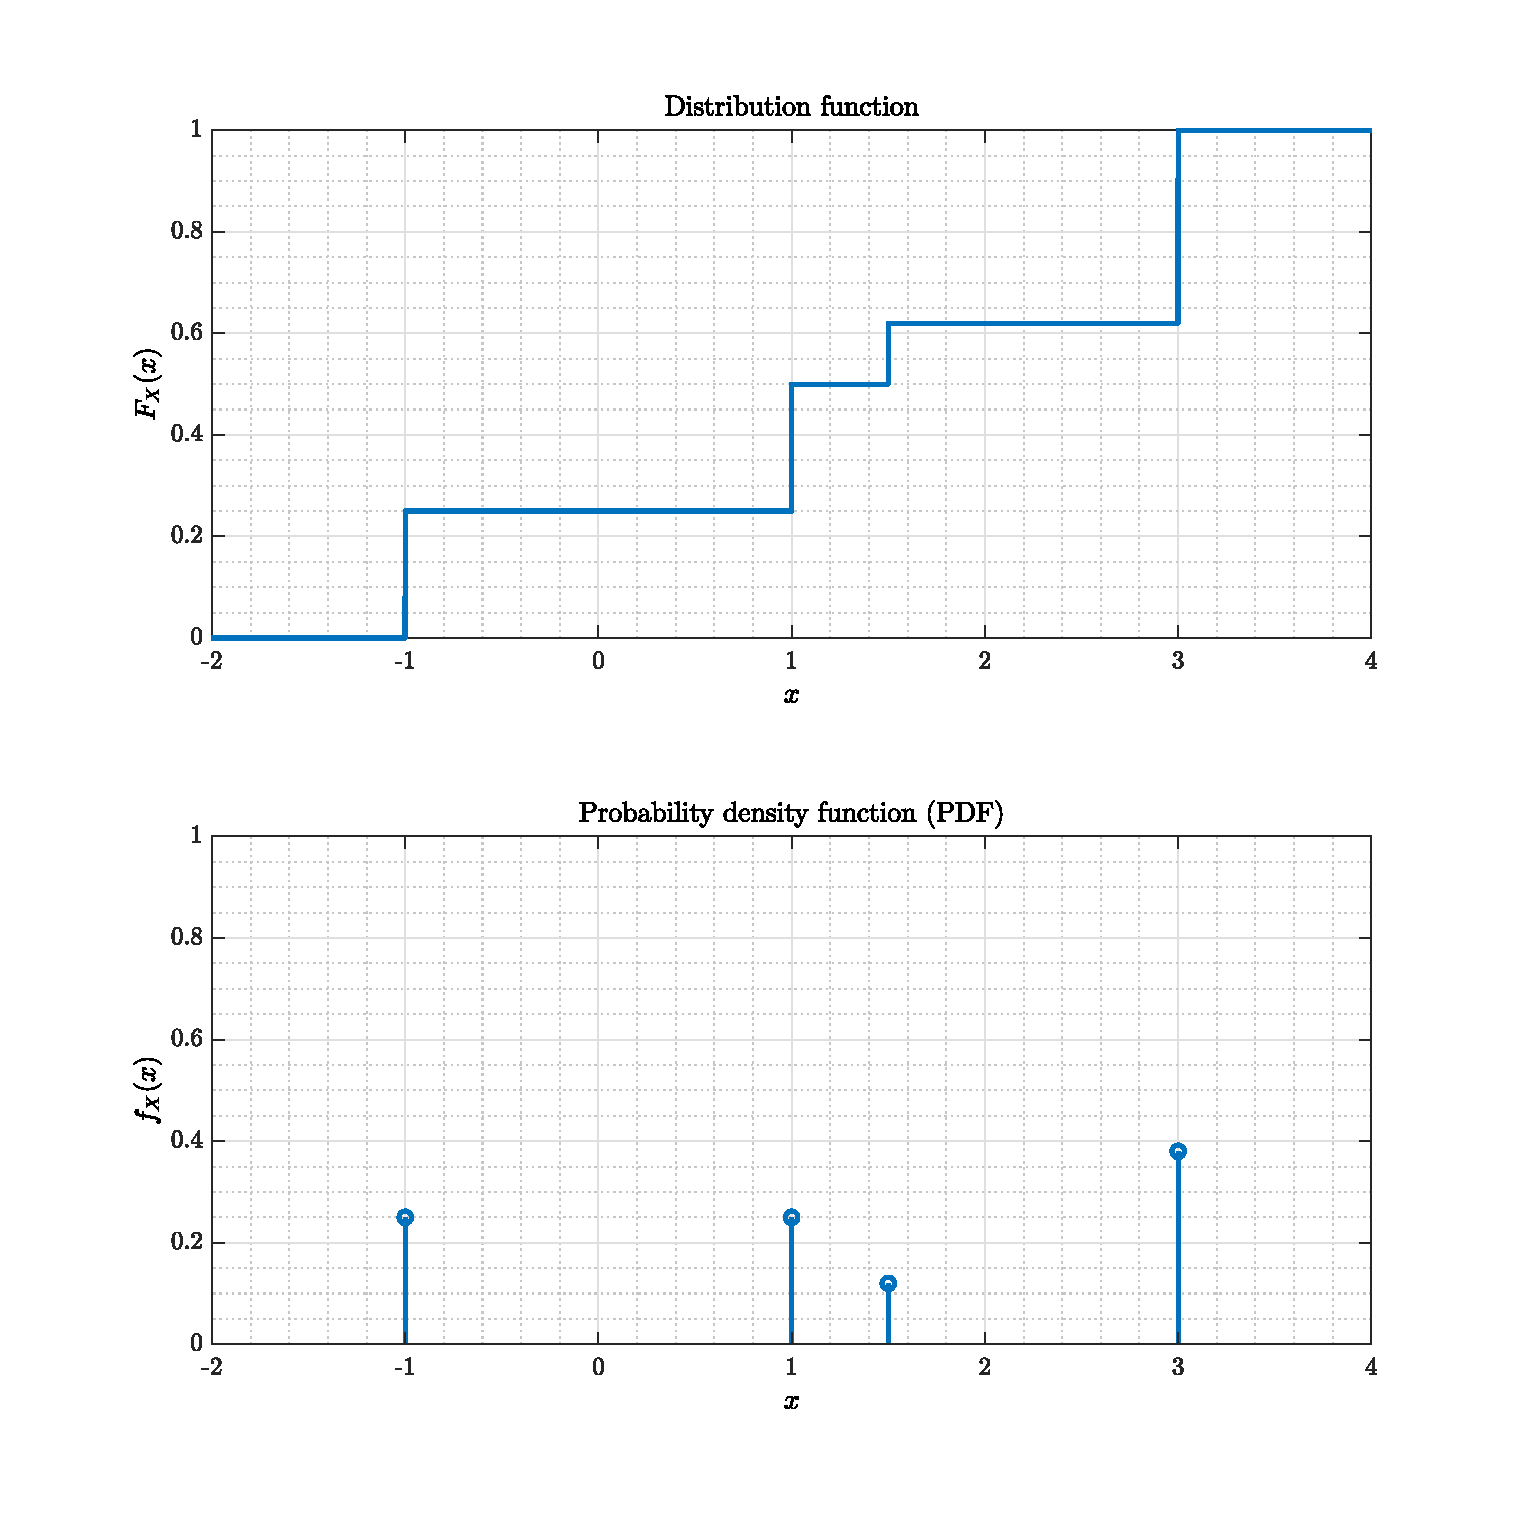
\includegraphics[width=12cm]{ej1.eps}
		\caption{Plot of Distribution function and PDF.}
		\label{fig:ej1}
	\end{figure}
			
	
	
	
	\item Random variable $X$ is uniform in the interval $[-1,3]$.
	\begin{enumerate}[a.]
		\item Find and plot density and distribution.
		\item Find the probability that rv $X$ is less than 2.
		\item Find the probability that rv $X$ is equal to 0.
	\end{enumerate}
	
	
	\textbf{Solution:}
	
	Knowing that $X$ is a uniform rv then we can use the following equation:
	\begin{equation}
		f_{X}(x)= \left\{ \begin{array}{lcl}
				\frac{1}{x_{2} - x_{1}} & \mbox{ if } & x_{1} \leq x  \leq x_{2}\\
				& & \\
				0 & \mbox{  } & \text{otherwise}
			\end{array}
		\right.
	\end{equation}
	
	then in our problem:

	\begin{tcolorbox}
	\begin{equation}
		f_{X}(x)= \left\{ \begin{array}{lcl}
				\frac{1}{4} & \mbox{ if } & -1 \leq x  \leq 3\\
				& & \\
				0 & \mbox{  } & \text{otherwise}
			\end{array}
		\right.
	\end{equation}
	\end{tcolorbox}
	
	then we can find the distribution function as follow:
	
	\begin{equation}
	 F_{X}(x) = \int_{-\infty}^{x} \frac{1}{4} dx = \frac{1}{4}x \biggr|^{x}_{-1} = \frac{1}{4}(x-1) \qquad \text{for} \qquad -1 \leq x  \leq 3
	 \end{equation}
	 then
	 
	 \begin{tcolorbox}
	\begin{equation}
		F_{X}(x)= \left\{ \begin{array}{lcl}
				1 & \mbox{ if } &  x  > 3\\
				& & \\
				\frac{1}{4}(x-1) & \mbox{ if } & -1 \leq x  \leq 3\\
				& & \\
				0 & \mbox{  } & \text{otherwise}
			\end{array}
		\right.
	\end{equation}
	\end{tcolorbox}
	 
	 The probability that $X < 2$ can be obtain computing the integral or simply evaluating in $f_{X}(x)$ with $x =2$, then:
	 
	 \begin{tcolorbox}
	\begin{equation}
		P\{ X < 2\} = F_{X}(2) = \frac{3}{4} = 0.75
	\end{equation}
	\end{tcolorbox}
	
	this result is consistent if we integrate the PDF function from $-\infty$ to $2$.
	
	The probability that $X = 0$ is zero, because for a continuous rv the probability that takes a particular value is zero. If we want to confirm this we can do the following:
	\begin{tcolorbox}
	\begin{equation}
	P\{ 0 < X \leq 0\} = P\{ X = 0\} = F_{X}(0) - F_{X}(0) = 0
	\end{equation}
	\end{tcolorbox}
	
	\begin{figure}[h!]
		\centering
		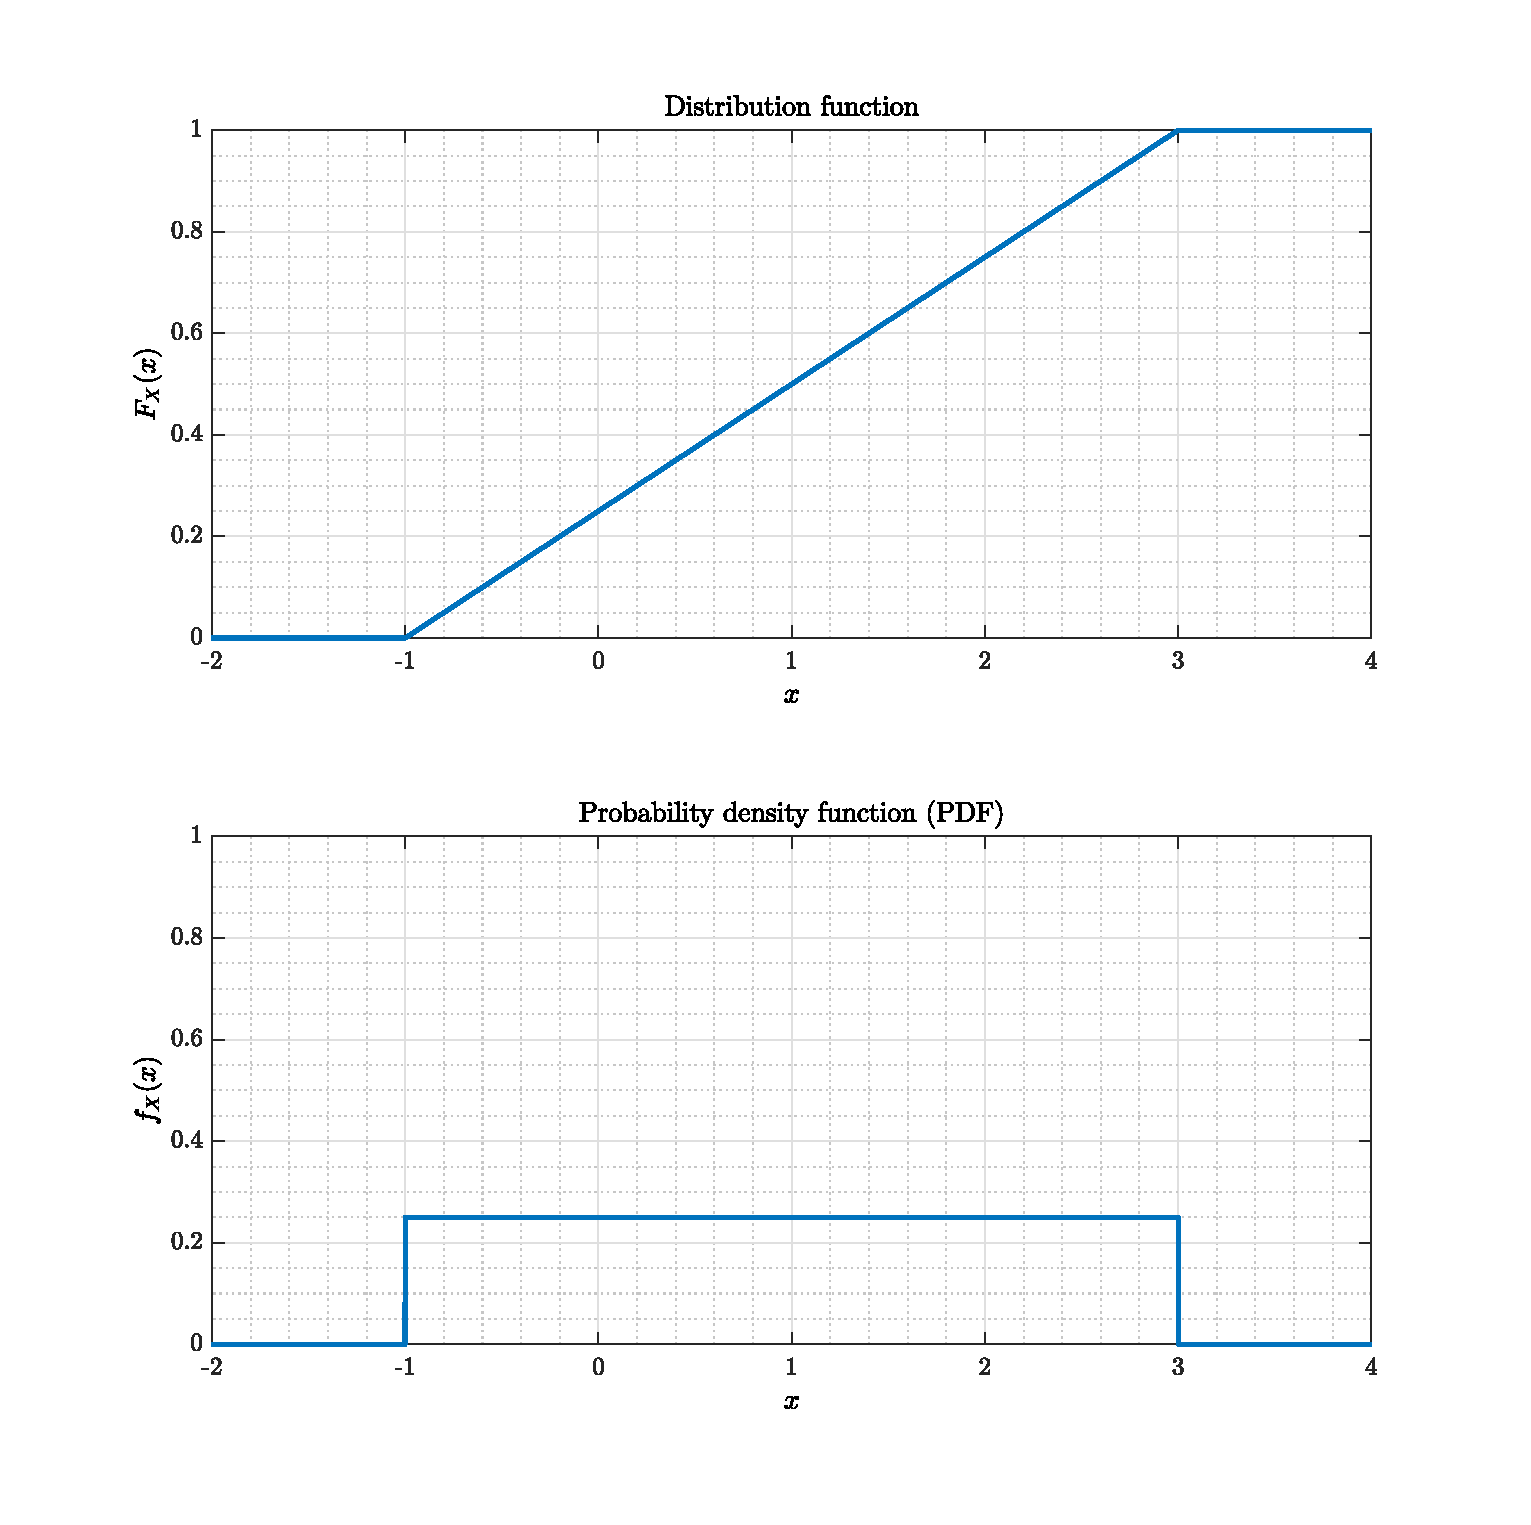
\includegraphics[width=12cm]{ej2.eps}
		\caption{Plot of Distribution function and PDF.}
		\label{fig:ej2}
	\end{figure}
	
	In Figure \ref{fig:ej2} we have the plots.
	
	\item Generate a uniform rv $X$ in the interval $[0,1]$ using the  \textbf{rand.m} function.
	\begin{enumerate}[a.]
		\item Find the density and distribution of the rv $X$.
		\item Plot histogram, probabilities in cell, and estimated PDF taking $N = 10000$ values and 20 cells.
		\item Plot estimated distribution.
	\end{enumerate}
	
	
	\textbf{Solution:}
	
	
	
	
	\begin{tcolorbox}
	\begin{equation}
		f_{X}(x)= \left\{ \begin{array}{lcl}
				1 & \mbox{ if } & 0 \leq x  \leq 1\\
				& & \\
				0 & \mbox{  } & \text{otherwise}
			\end{array}
		\right.
	\end{equation}
	\end{tcolorbox}
	
	 
	 \begin{tcolorbox}
	\begin{equation}
		F_{X}(x)= \left\{ \begin{array}{lcl}
				1 & \mbox{ if } &  x  > 1\\
				& & \\
				x & \mbox{ if } & 0 \leq x  \leq 1\\
				& & \\
				0 & \mbox{  } & \text{otherwise}
			\end{array}
		\right.
	\end{equation}
	\end{tcolorbox}	
	
	
	
	\begin{figure}[h!]
		\centering
		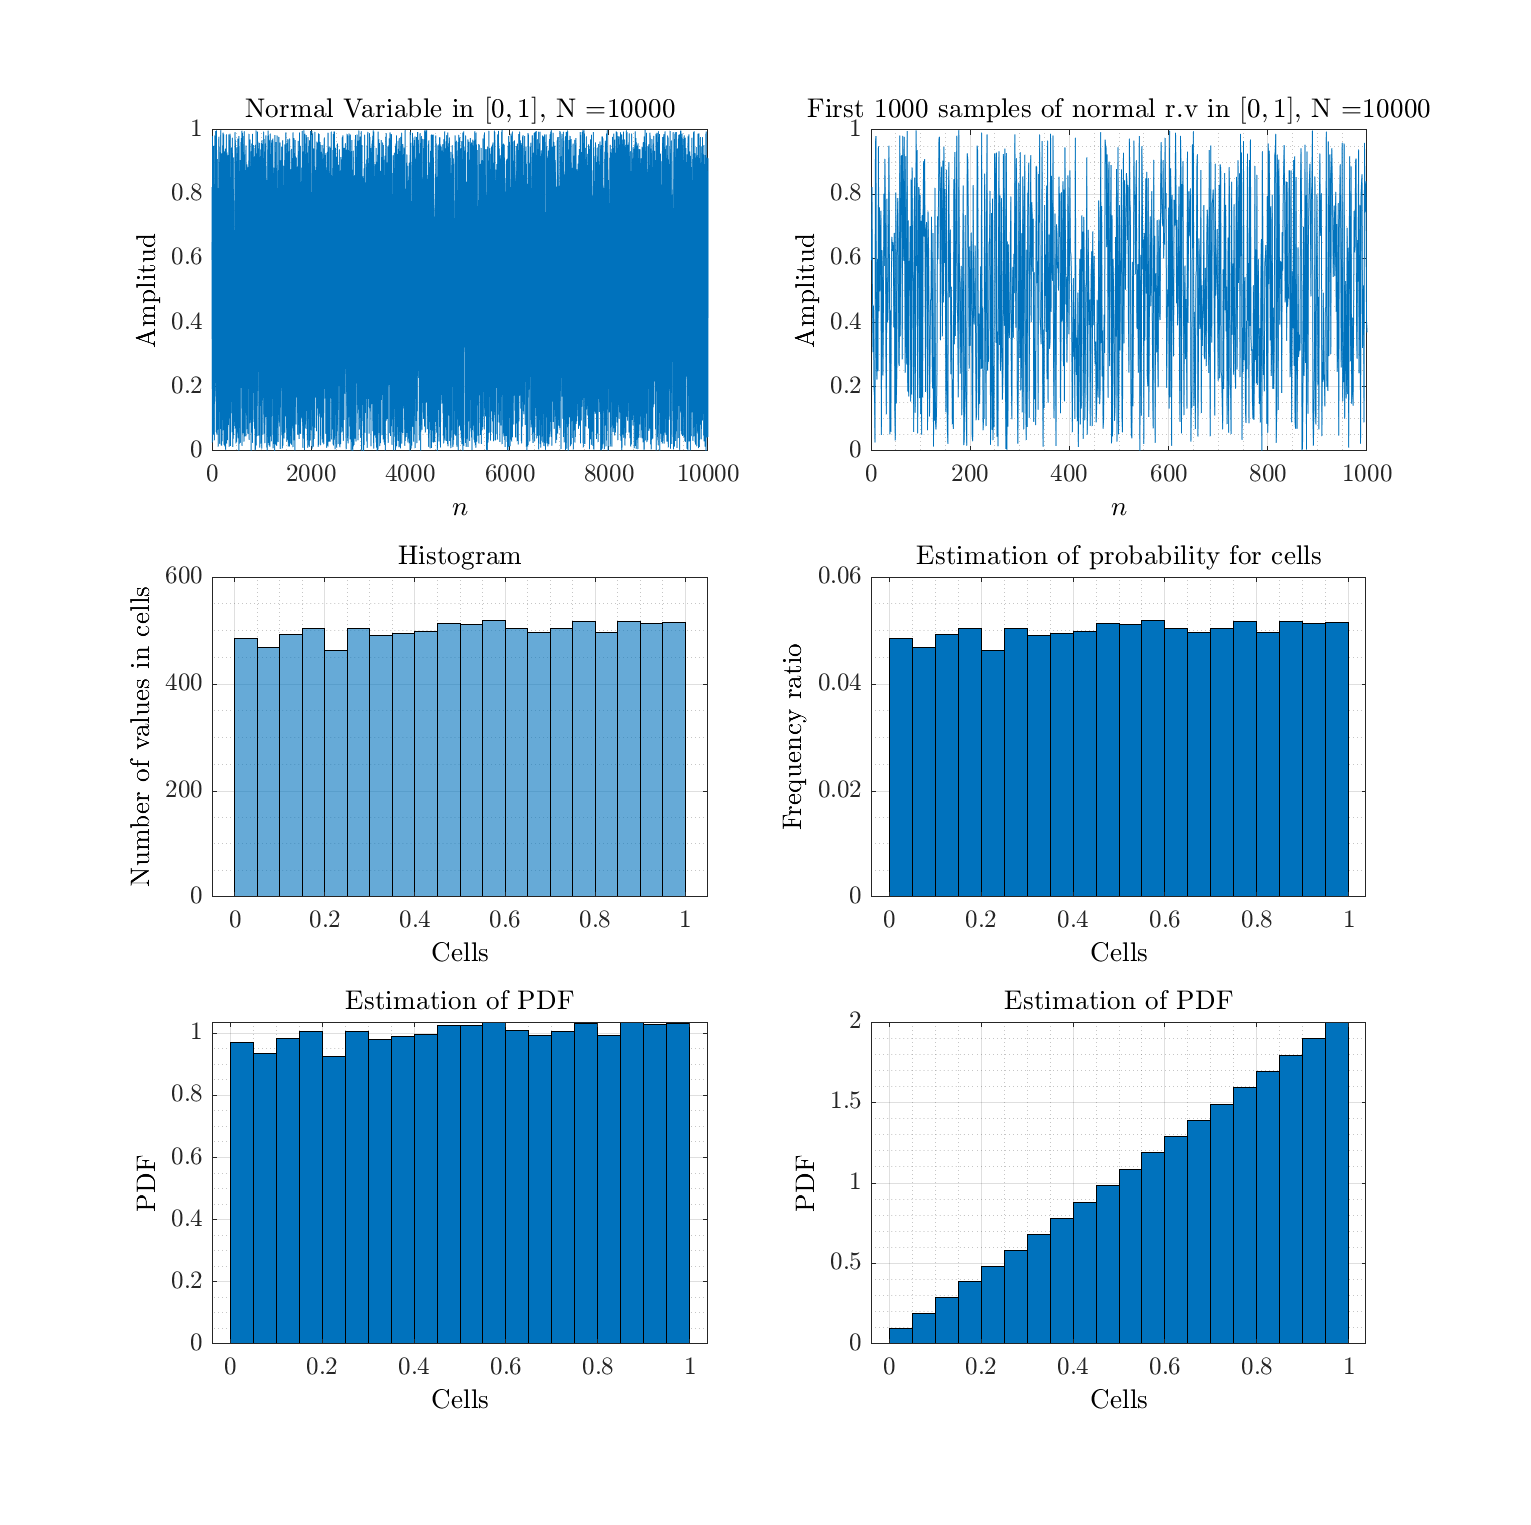
\includegraphics[width=15cm]{ej3.eps}
		\caption{Complete analysis of normal rv.}
	\end{figure}
	
	
	
\end{enumerate}



\newpage

\lstinputlisting[style = MATLAB, caption =  Solve problem 1., label = cod:ej1]{ej1.m}


\lstinputlisting[style = MATLAB, caption =  Solve problem 2., label = cod:ej2]{ej2.m}

\lstinputlisting[style = MATLAB, caption =  Solve PDF and distribution., label = cod:pdf]{PDF_custom.m}

\begin{thebibliography}{99}
\bibitem{gordana} Random Signals and Processes Primer with MATLAB. Gordana Jocanovic Dolecek.
\end{thebibliography}


\end{document}